\lab{Nearest Neighbor Search}{Nearest Neighbor Search}

\objective{The nearest neighbor problem is an optimization problem that arises in applications such as computer vision, internet marketing, and data compression.
The problem can be solved efficiently with a $k$-d tree, a generalization of the binary search tree.
In this lab we implement a $k$-d tree, use it to solve the nearest neighbor problem, then use that solution as the basis of an elementary machine learning algorithm.}

\section*{The Nearest Neighbor Problem} % =====================================

Let $X \subset \mathbb{R}^k$ be a collection of data, called the \emph{training set}, and let $\z \in \mathbb{R}^k$, called the \emph{target}.
The \emph{nearest neighbor search problem} is determining the point $\x^* \in X$ that is ``closest'' to $\z$.

For example, suppose you move into a new city with several post offices.
Since your time is valuable, you wish to know which post office is closest to your home.
The set $X$ could be addresses or latitude and longitude data for each post office in the city; $\z$ would be the data that represents your new home.
The task is to find the closest post office in $\x \in X$ to your home $\z$.

\subsection*{Metrics and Distance} % ------------------------------------------

Solving the nearest neighbor problem requires a definition for distance between $\z$ and elements of $X$.
In $\mathbb{R}^k$, distance is typically defined by the \emph{Euclidean metric}.
\begin{align}
\label{eq:nearest-neighbor-euclidean-metric}
d(\x,\z) = \|\x - \z\| = \sqrt{\sum_{i=1}^k(x_i-z_i)^2}
\end{align}
Here $\|\cdot\|$ is the standard \emph{Euclidean norm}, which computes vector length.
In other words, $d(\x,\z)$ is the length of the straight line from $\x$ to $\z$.
With this notation, the nearest neighbor search problem can be written as follows.
\begin{align}
\label{eq:nearest-neighbor-def}
\x^* = \underset{\x\in X}{\text{argmin}}\:d(\x,\z)
\qquad\qquad
d^* = \min_{\x\in X}d(\x,\z)
\end{align}

NumPy and SciPy implement the Euclidean norm (and other norms) in \li{linalg.norm()}.
This function accepts vectors or matrices.
Use the \li{axis} argument to compute the norm along the rows or columns of a matrix: \li{axis=0} computes the norm of each column, and \li{axis=1} computes the norm of each row (see the NumPy Visual Guide).

\begin{lstlisting}
>>> import numpy as np
>>> from scipy import linalg as la

>>> x0 = np.array([1, 2, 3])
>>> x1 = np.array([6, 5, 4])

# Calculate the length of the vectors x0 and x1 using the Euclidean norm.
>>> la.norm(x0)
3.7416573867739413
>>> la.norm(x1)
8.7749643873921226

# Calculate the distance between x0 and x1 using the Euclidean metric.
>>> la.norm(x0 - x1)
5.9160797830996161

>>> A = np.array([[1, 2, 3],        # or A = np.vstack((x0,x1)).
...               [6, 5, 4]])
>>> la.norm(A, axis=0)              # Calculate the norm of each column of A.
array([ 6.08276253,  5.38516481,  5.        ])
>>> la.norm(A, axis=1)              # Calculate the norm of each row of A.
array([ 3.74165739,  8.77496439])   # This is ||x0|| and ||x1||.
\end{lstlisting}

\subsection*{Exhaustive Search} % ---------------------------------------------

Consider again the post office example.
One way to find out which post office is closest is to drive from home to each post office, measuring the distance travelled in each trip.
That is, we solve \eqref{eq:nearest-neighbor-def} by computing $\|\x - \z\|$ for every point $\x\in X$.
This strategy is called a \emph{brute force} or \emph{exhaustive search}.

\begin{problem} % Exhaustive search method.
Write a function that accepts a $m\times k$ NumPy array $X$ (the training set) and a 1-dimensional NumPy array $\z$ with $k$ entries (the target).
Each of the $m$ rows of $X$ represents a point in $\mathbb{R}^k$ that is an element of the training set.

Solve \eqref{eq:nearest-neighbor-def} with an exhaustive search.
Return the nearest neighbor $\x^*$ and its Euclidean distance $d^*$ from the target $\z$.
\\(Hint: use array broadcasting and the \li{axis} argument to avoid using a loop.)
\label{prob:nearest-neighbor-exhaustive-search}
\end{problem}

The complexity of an exhaustive search for $X\subset\mathbb{R}^k$ with $m$ points is $O(km)$, since \eqref{eq:nearest-neighbor-euclidean-metric} is $O(k)$ and there are $m$ norms to compute.
This method works, but it is only feasible for relatively small training sets.
Solving the problem with greater efficiency requires the use of a specialized data structure.

\section*{K-D Trees} % ========================================================

% \footnote{This lab is a sequel to the Data Structures II lab, and should not be attempted until the reader has successfully implemented a binary search tree in Python.}
A \href{https://en.wikipedia.org/wiki/K-d_tree}{\emph{$k$-d tree}} is a generalized binary search tree where each node in the tree contains $k$-dimensional data.
Just as a BST makes searching easy in $\mathbb{R}$, a $k$-d tree provides a way to efficiently search $\mathbb{R}^k$.

A BST creates a partition of $\mathbb{R}$: if a node contains the value $x$, all of the nodes in its left subtree contain values that are less than $x$, and the nodes of its right subtree have values that are greater than $x$.
Similarly, a $k$-d tree partitions $\mathbb{R}^k$.
Each node is assigned a \emph{pivot} value $i \in \{0,1,\ldots,k-1\}$ corresponding to the depth of the node: the root has $i=0$, its children have $i=1$, their children have $i=2$, and so on.
If a node has $i=k-1$, its children have $i=0$, their children have $i=1$, and so on.
% In general, if a node has \li{pivot} $i$, its children have an \li{pivot} of $(i + 1) \mod k$.
The tree is constructed such that for a node containing $\x = [x_0,x_1,\ldots,x_{k-1}]\trp \in\mathbb{R}^k$, if a node in the left subtree contains $\y$, then $y_i < x_i$.
Conversely, if a node in the right subtree contains $\z$, then $x_i \le z_i$.
See Figure \ref{fig:nearest-neighbor-pivot-tree} for an example where $k = 3$.

% The case where $k=1$ results in a usual BST, since each value in the tree is a member of $\mathbb{R}$.

\begin{figure}[H] % 3-d tree with pivot entries marked.
\begin{tikzpicture}[
    level 1/.style={sibling distance=7cm},
    level 2/.style={sibling distance=4cm},
    level 3/.style={sibling distance=3cm},
    level 4/.style={sibling distance=3cm},
    edge from parent/.style={draw, ->,thick, >=stealth'}]

    % Place the nodes and labels
    \node [thick,circle,draw] (a) {$[\textcolor{red}{3},1,4]$}
        child {node[thick,circle,draw] (b) {$[1,\textcolor{red}{2},7]$}
            child {node[thick,circle,draw] (c) {$[2,0,\textcolor{red}{3}]$}}
            child {node[thick,circle,draw] (d) {$[2,4,\textcolor{red}{5}]$}
                child {node[thick,circle,draw] (e) {$[\textcolor{red}{1},4,3]$}}
                child {node[thick,circle,draw] (f) {$[\textcolor{red}{0},5,7]$}}}}
        child {node[thick,circle,draw] (g) {$[4,\textcolor{red}{3},5]$}
            child {node[thick,circle,draw] (h) {$[6,1,\textcolor{red}{4}]$}
                child {node[draw = none] (invisble) {} edge from parent[draw=none]}
                child {node[thick,circle,draw] (i) {$[\textcolor{red}{5},2,5]$}}}
            child {node[draw = none] (invisble1) {} edge from parent[draw=none]}};

    % pivot labels
    \node [draw=none,red,node distance=5.7cm]  (1) [right of=a] {\li{pivot=0}};
    \node [draw=none,red,node distance=2.18cm] (2) [right of=g] {\li{pivot=1}};
    \node [draw=none,red,node distance=4.19cm] (3) [right of=h] {\li{pivot=2}};
    \node [draw=none,red,node distance=2.69cm] (4) [right of=i] {\li{pivot=0}};
\end{tikzpicture}

\caption{A $k$-d tree with $k = 3$.
The root $[\textcolor{red}{3},1,4]$ has an \li{pivot} of $0$, so $[1,2,7]$ is to the left of the root because $1<\textcolor{red}{3}$, and $[4,3,5]$ is to the right since $\textcolor{red}{3} \le 4$.
Similarly, the node $[2,4,\textcolor{red}{5}]$ has an \li{pivot} of $2$, so $[1,4,3]$ is to its left since $4<\textcolor{red}{5}$ and $[0,5,7]$ is to its right because $\textcolor{red}{5}\le 7$.
The nodes that are furthest from the root have an \li{pivot} of $0$ because their parents have an \li{pivot} of $2 = k - 1$.}
\label{fig:nearest-neighbor-pivot-tree}
\end{figure}

\begin{problem} % Write a KDTNode class from scratch.
Write a \li{KDTNode} class whose constructor accepts a single parameter $\x \in \mathbb{R}^k$.
If $\x$ is not a NumPy array (of type \li{np.ndarray}), raise a \li{TypeError}.
Save $\x$ as an attribute called \li{value}, and initialize attributes \li{left}, \li{right}, and \li{pivot} as \li{None}.
The \li{pivot} will be assigned when the node is inserted into the tree, and \li{left} and \li{right} will refer to child nodes.
\end{problem}

% Now we construct the $k$-d tree class.
% For an optimal $k$-d tree, the data needs to be inserted in a very particular order.
% However, inserting at random still usually produces a good tree.
% Here we simply insert the data in the order that it is given.
% TODO: put this elsewhere (in the problem statement?).

\subsection*{Constructing the Tree} % -----------------------------------------

\subsubsection*{Locating Nodes} % - - - - - - - - - - - - - - - - - - - - - - -

The \li{find()} methods for $k$-d trees and binary search trees are very similar.
Both recursively compare the values of a target and nodes in the tree, but in a $k$-d tree, these values must be compared according to their \li{pivot} attribute.
% Solving the nearest neighbor problem does not require a \li{find()} method, the $k$-d tree version of \li{find()} is provided as an instructive example.
Every comparison in the recursive \li{_step()} function, implemented below, compares the data of \li{target} and \li{current} based on the \li{pivot} attribute of \li{current}.
See Figure \ref{fig:nearest-neighbor-kdfind}.

\begin{lstlisting}
class KDT:
    """A k-dimensional tree for solving the nearest neighbor problem.

    Attributes:
        root (KDTNode): the root node of the tree. Like all other nodes in
            the tree, the root has a NumPy array of shape (k,) as its value.
        k (int): the dimension of the data in the tree.
    """
    def __init__(self):
        """Initialize the root and k attributes."""
        self.root = None
        self.k = None

    def find(self, data):
        """Return the node containing the data. If there is no such node in
        the tree, or if the tree is empty, raise a ValueError.
        """
        def _step(current):
            """Recursively step through the tree until finding the node
            containing the data. If there is no such node, raise a ValueError.
            """
            if current is None:                     # Base case 1: dead end.
                raise ValueError(str(data) + " is not in the tree")
            elif np.allclose(data, current.value):
                return current                      # Base case 2: data found!
            elif data[current.pivot] < current.value[current.pivot]:
                return _step(current.left)          # Recursively search left.
            else:
                return _step(current.right)         # Recursively search right.

        # Start the recursive search at the root of the tree.
        return _step(self.root)
\end{lstlisting}

\begin{figure}[H]
\begin{tikzpicture}[
    level 1/.style={sibling distance=7cm},
    level 2/.style={sibling distance=4cm},
    level 3/.style={sibling distance=3cm},
    level 4/.style={sibling distance=3cm},
    edge from parent/.style={draw, ->,thick, >=stealth'}]

    % Place the nodes and labels
    \node [draw=blue, circle,fill=blue!10!,thick] (a) {$[\textcolor{red}{3},1,4]$}
        child {node[draw=blue, circle, fill=blue!10!,thick] (b) {$[1,\textcolor{red}{2},7]$}
            child {node[thick,circle,draw] (c) {$[2,0,\textcolor{red}{3}]$}}
            child {node[draw=blue, circle,thick,fill=blue!10!] (d) {$[2,4,\textcolor{red}{5}]$}
                child {node[draw=blue, circle,thick,fill=blue!10!] (e) {$[\textcolor{red}{1},4,3]$}}
                child {node[thick,circle,draw] (f) {$[\textcolor{red}{0},5,7]$}}}}
        child {node[thick,circle,draw] (g) {$[4,\textcolor{red}{3},5]$}
            child {node[thick,circle,draw] (h) {$[6,1,\textcolor{red}{4}]$}
                child {node[draw = none] (invisble) {} edge from parent[draw=none]}
                child {node[thick,circle,draw] (i) {$[\textcolor{red}{5},2,5]$}}}
            child {node[draw = none] (invisble1) {} edge from parent[draw=none]}};
    \draw [blue!100!,->,thick,>=stealth'] (a)--(b);
    \draw [blue!100!,->,thick,>=stealth'] (b)--(d);
    \draw [blue!100!,->,thick,>=stealth'] (d)--(e);

    % pivot labels
    \node [draw=none,red,node distance=5.7cm]  (1) [right of=a] {\li{pivot=0}};
    \node [draw=none,red,node distance=2.18cm] (2) [right of=g] {\li{pivot=1}};
    \node [draw=none,red,node distance=4.19cm] (3) [right of=h] {\li{pivot=2}};
    \node [draw=none,red,node distance=2.69cm] (4) [right of=i] {\li{pivot=0}};
\end{tikzpicture}
\caption{To locate the node containing $[1,4,3]$, start by comparing $[1,4,3]$ to the root $[\textcolor{red}{3},1,4]$.
The root has an \li{pivot} of $0$, so compare the first component of the data to the first component of the root: since $1<\textcolor{red}{3}$, step left.
Next, $[1,4,3]$ must be to the right of $[1,\textcolor{red}{2},7]$ because $\textcolor{red}{2}\le 4$.
Similarly, $[1,4,3]$ must be to the left of $[2,4,\textcolor{red}{5}]$ as $3<\textcolor{red}{5}$.} %, where the node containing $[1,4,3]$ is found.}
\label{fig:nearest-neighbor-kdfind}
\end{figure}

\begin{figure}[H] % KDT.insert()
\captionsetup[subfigure]{justification=justified}
\begin{center}
\begin{subfigure}{\textwidth}
    \centering
    \begin{tabular}{lcr}
    \begin{tikzpicture}[
        baseline=(current bounding box.south),
        level 1/.style={sibling distance=4cm, level distance=1cm},
        level 2/.style={sibling distance=2.5cm, level distance=1cm},
        level 3/.style={sibling distance=1.5cm, level distance=1cm},
        edge from parent/.style={draw, ->, thick, >=stealth'}]
        \node [thick,circle,draw] (a) {$[\textcolor{red}{5},5]$}
          child {node[draw=none] (b) {\textcolor{gray}{$A$}} edge from parent[draw=gray]
            child {node[draw=none] (d) {} edge from parent[draw=none]}
            child {node[draw=none] (e) {} edge from parent[draw=none]
                child {node[draw=none] (i) {} edge from parent[draw=none]}
                child {node[draw=none] (j) {} edge from parent[draw=none]}}}
          child {node[draw=none] (b) {\textcolor{gray}{$B$}} edge from parent[draw=gray]
            child {node[draw=none] (f) {} edge from parent[draw=none]}
            child {node[draw=none] (g) {} edge from parent[draw=none]}};
    \end{tikzpicture}
    &\textcolor{white}{----------}&\textcolor{white}{[]}
    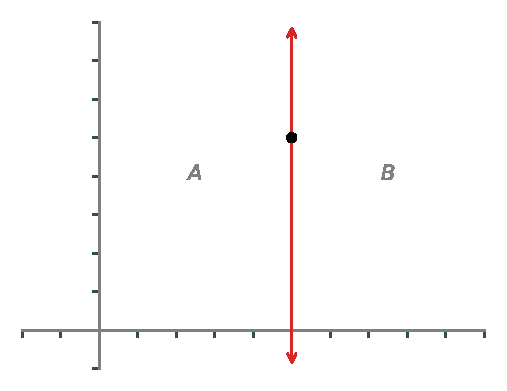
\includegraphics[width=.4\textwidth]{figures/partition1.pdf}
    \end{tabular}
    \caption{Insert $[5,5]$ as the root.
    The root always has an \li{pivot} of $0$, so nodes to the left of the root contain points from $A = \{(x,y)\in\mathbb{R}^2 : x < \textcolor{red}{5}\}$, and nodes on the right branch have points in $B = \{(x,y)\in\mathbb{R}^2 : \textcolor{red}{5}\le x\}$.}
\end{subfigure}
\begin{subfigure}{\textwidth}
    \centering
    \begin{tabular}{lcr}
    \begin{tikzpicture}[
        baseline=(current bounding box.south),
        level 1/.style={sibling distance=4cm, level distance=1cm},
        level 2/.style={sibling distance=2.5cm, level distance=1cm},
        level 3/.style={sibling distance=1.5cm, level distance=1cm},
        edge from parent/.style={draw, ->, thick, >=stealth'}]
        \node [thick,circle,draw] (a) {$[\textcolor{red}{5},5]$}
          child {node[thick,circle,draw] (b) {$[3,\textcolor{blue}{2}]$}
            child {node[draw=none] (d) {\textcolor{gray}{$A$}} edge from parent[draw=gray]}
            child {node[draw=none] (e) {\textcolor{gray}{$B$}} edge from parent[draw=gray]
                child {node[draw=none] (i) {} edge from parent[draw=none]}
                child {node[draw=none] (j) {} edge from parent[draw=none]}}}
          child {node[thick,circle,draw] (b) {$[8,\textcolor{blue}{4}]$}
            child {node[draw=none] (f) {\textcolor{gray}{$C$}} edge from parent[draw=gray]}
            child {node[draw=none] (g) {\textcolor{gray}{$D$}} edge from parent[draw=gray]}};
    \end{tikzpicture}
    &\textcolor{white}{----------}&
    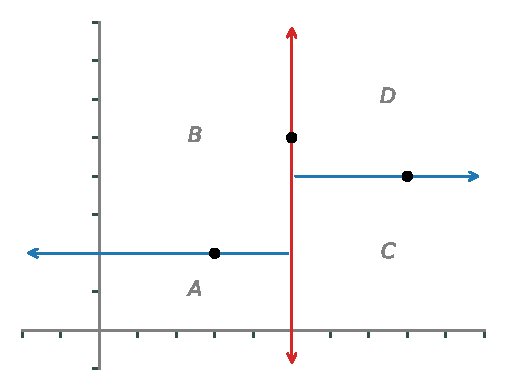
\includegraphics[width=.4\textwidth]{figures/partition2.pdf}
    \end{tabular}
    \caption{Insert $[3,2]$, then $[8,4]$.
    Since $3 < \textcolor{red}{5}$, $[3,2]$ becomes the left child of $[\textcolor{red}{5},5]$.
    Likewise, as $\textcolor{red}{5}\le 8$, $[8,4]$ becomes the right child of $[\textcolor{red}{5},5]$.
    These new nodes have an \li{pivot} of $1$, so they partition the space vertically:
    nodes to the right of $[3,\textcolor{blue}{2}]$ contain points from $B = \{(x,y)\in\mathbb{R}^2 : x < \textcolor{red}{5},\ \textcolor{blue}{2} \le y\}$;
    nodes to the left of $[8,\textcolor{blue}{4}]$ hold points from $C = \{(x,y)\in\mathbb{R}^2 : \textcolor{red}{5} \le x,\ y < \textcolor{blue}{8}\}$.}
\end{subfigure}
\begin{subfigure}{\textwidth}
    \centering
    \begin{tabular}{lcr}
    \begin{tikzpicture}[
        baseline=(current bounding box.south),
        level 1/.style={sibling distance=4cm, level distance=1cm},
        level 2/.style={sibling distance=2.5cm, level distance=1cm},
        level 3/.style={sibling distance=1.5cm, level distance=1cm},
        edge from parent/.style={draw, ->, thick, >=stealth'}]
        \node [thick,circle,draw] (a) {$[\textcolor{red}{5},5]$}
            child {node[thick,circle,draw] (b) {$[3,\textcolor{blue}{2}]$}
                child {node[draw=none] (d) {\textcolor{gray}{$A$}} edge from parent[draw=gray]}
                child {node[thick,circle,draw] (e) {$[\textcolor{red}{2},6]$}
                  child {node[draw=none] (i) {\textcolor{gray}{$B$}} edge from parent[draw=gray]}
                  child {node[draw=none] (j) {\textcolor{gray}{$C$}} edge from parent[draw=gray]}}}
            child {node[thick,circle,draw] (c) {$[8,\textcolor{blue}{4}]$}
                child {node[draw=none] (f) {\textcolor{gray}{$D$}} edge from parent[draw=gray]}
                child {node[draw=none] (g) {\textcolor{gray}{$E$}} edge from parent[draw=gray]}};
    \end{tikzpicture}
    &\textcolor{white}{----------}&
    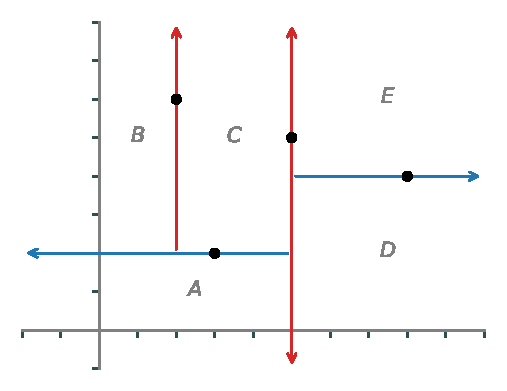
\includegraphics[width=.4\textwidth]{figures/partition3.pdf}
    \end{tabular}
    \caption{Insert $[2,6]$.
    The \li{pivot} cycles back to $0$ since $k = 2$, so nodes to the left of $[\textcolor{red}{2},6]$ have points that lie in $B = \{(x,y)\in\mathbb{R}^2 : x < \textcolor{red}{2},\ \textcolor{blue}{2} \le y\}$
    and nodes to the right store points in $C = \{(x,y)\in\mathbb{R}^2 : \textcolor{red}{2} \le x < \textcolor{red}{5},\ \textcolor{blue}{2} \le y\}$.}
\end{subfigure}
\end{center}
\caption{As a $k$-d tree is constructed (left), it creates a partition of $\mathbb{R}^k$ (right) by defining separating hyperplanes that pass through the points.
The more points, the finer the partition.}
\label{fig:nearest-neighbor-KDT_insert}
\end{figure}

\subsubsection*{Inserting Nodes} % - - - - - - - - - - - - - - - - - - - - - -

% New nodes in a $k$-d tree are always added as leaf nodes.
To add a new node to a $k$-d tree, determine which existing node should be the parent of the new node by recursively stepping down the tree as in the \li{find()} method.
Next, assign the new node as the \li{left} or \li{right} child of the parent, and set its \li{pivot} based on its parent's \li{pivot}: if the parent's \li{pivot} is $i$, the new node's \li{pivot} should be $i+1$, or $0$ if $i = k-1$.

Consider again the $k$-d tree in Figure \ref{fig:nearest-neighbor-kdfind}.
To insert $[2,3,4]$, search the tree for $[2,3,4]$ until hitting an empty slot.
In this case, the search steps from the root down to $[\textcolor{red}{1},4,3]$, which has an \li{pivot} of $0$.
Then since $\textcolor{red}{1} \le 2$, the new node should be to the right of $[1,4,3]$.
However, $[\textcolor{red}{1},4,3]$ has no right child, so it becomes the parent of $[2,3,4]$.
The \li{pivot} of the new node should therefore be $1$.
See Figure \ref{fig:nearest-neighbor-KDT_insert} for another example.
% This method partitions $\mathbb{R}^k$ into smaller subsections, allowing for efficient searching.

\begin{problem} % KDT.insert()
\label{prob:kdt-insert}
Write an \li{insert()} method for the \li{KDT} class that accepts a point $\x\in\mathbb{R}^k$.
\begin{enumerate}
\item If the tree is empty, create a new \li{KDTNode} containing $\x$ and set its \li{pivot} to $0$.
Assign the \li{root} attribute to the new node and set the \li{k} attribute as the length of $\x$.
Thereafter, raise a \li{ValueError} if data to be inserted is not in $\mathbb{R}^k$.
\item If the tree is nonempty, create a new \li{KDTNode} containing $\x$ and find the existing node that should become its parent.
Determine whether the new node will be the parent's \li{left} or \li{right} child, then link the parent to the new node accordingly.
Set the \li{pivot} of the new node based on its parent's \li{pivot}.
\\(Hint: write a recursive function like \li{_step()} to find and link the parent.)
\item Do not allow duplicates in the tree: if there is already a node in the tree containing $\x$, raise a \li{ValueError}.
% Be careful to check the entire array, not just the \li{pivot} entry.
\end{enumerate}
To test your method, use the \li{__str__()} method provided in the Additional Materials section.
Try constructing the trees in Figures \ref{fig:nearest-neighbor-pivot-tree} and \ref{fig:nearest-neighbor-KDT_insert}.
Also check that the provided \li{find()} method works as expected.
\end{problem}

\subsection*{Nearest Neighbor Search with K-D Trees} % ------------------------

Given a target $\z\in\mathbb{R}^k$ and a $k$-d tree containing a set $X\subset\mathbb{R}^k$ of $m$ points, the nearest neighbor problem can be solved by traversing the tree in a manner that is similar to the \li{find()} or \li{insert()} methods from the previous section.
The advantage of this strategy over an exhaustive search is that not every $\x\in X$ has to be compared to $\z$ via \eqref{eq:nearest-neighbor-euclidean-metric}; the tree structure makes it possible to rule out some elements of $X$ without actually computing their distances to $\z$.
The complexity is $O(k\log(m))$, a significant improvement over the $O(km)$ complexity of an exhaustive search.

To begin, set $\x^*$ as the value of the root and compute $d^* = d(\x^*,\z)$.
Starting at the root, step down through the tree as if searching for the target $\z$.
At each step, determine if the value $\x$ of the current node is closer to $\z$ than $\x^*$.
If it is, assign $\x^* = \x$ and recompute $d^* = d(\x^*, \z)$.
Continue this process until reaching a leaf node.

Next, backtrack along the search path and determine if the non-explored branch needs to be searched.
To do this, check that the sphere of radius $d^*$ centered at $\z$ does not intersect with the separating hyperplane defined by the current node.
That is, if the separating hyperplane is further than $d^*$ from $\z$, then no points on the other side of the hyperplane can possibly be the nearest neighbor. %, so the branch that hasn't been searched can be safely ignored.
See Figure \ref{fig:nearest-neighbor-query} for an example and Algorithm \ref{alg:nearest-neighbor-search} for the details of the procedure.

\begin{figure}[H] % KDT.query()
\captionsetup[subfigure]{justification=justified}
\begin{center}
\begin{subfigure}{\textwidth}
    \centering
    \begin{tabular}{lcr}
    \begin{tikzpicture}[
        baseline=(current bounding box.south),
        level 1/.style={sibling distance=4cm, level distance=1cm},
        level 2/.style={sibling distance=2.5cm, level distance=1cm},
        level 3/.style={sibling distance=1.5cm, level distance=1.5cm},
        edge from parent/.style={draw, ->,thick, >=stealth'}]
        \node [draw=purple,thick,circle,fill=green!20!] (a) {$[\textcolor{red}{5},5]$}
          child {node[thick,circle,draw] (b) {$[3,\textcolor{blue}{2}]$}
            child {node[draw = none] (invisble) {} edge from parent[draw=none]}
            child {node[thick,circle,draw] (c) {$[\textcolor{red}{2},6]$}
              child {node[draw=none] (i) {} edge from parent[draw=none]}}}
          child {node[thick,circle,draw] (g) {$[8,\textcolor{blue}{4}]$}
            child {node[draw = none] (invisible1) {} edge from parent[draw=none]}
            child {node[draw,circle] (e) {$[\textcolor{red}{7},7]$}}};
    \end{tikzpicture}
    &\textcolor{white}{----------}&
    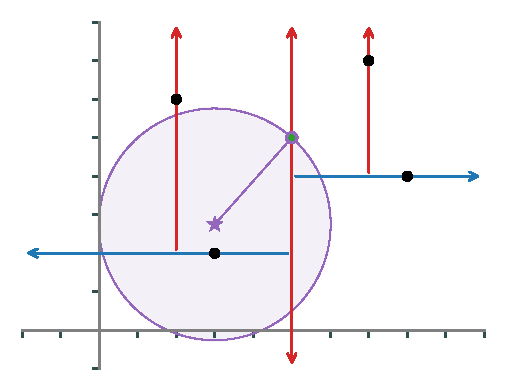
\includegraphics[width=.4\textwidth]{figures/kdtnn_search1.pdf}
    \end{tabular}
    \caption{Start at the root, setting $\x^* = [\textcolor{red}{5},5]$.
    The sphere of radius $d^* = d(\x^*,\z)$ centered at $\z$ intersects the hyperplane $x = 5$, so (at this point) it is possible that a nearer neighbor lies to the right of the root.}
\end{subfigure}
\begin{subfigure}{\textwidth}
    \centering
    \begin{tabular}{lcr}
    \begin{tikzpicture}[
        baseline=(current bounding box.south),
        level 1/.style={sibling distance=4cm, level distance=1cm},
        level 2/.style={sibling distance=2.5cm, level distance=1cm},
        level 3/.style={sibling distance=1.5cm, level distance=1.5cm},
        edge from parent/.style={draw, ->,thick, >=stealth'}]
        \node [thick,circle,draw] (a) {$[\textcolor{red}{5},5]$}
          child {node[draw=purple,thick,circle,fill=green!20!] (b) {$[3,\textcolor{blue}{2}]$} edge from parent[draw=red]
            child {node[draw = none] (invisble) {} edge from parent[draw=none]}
            child {node[thick,circle,draw=black] (c) {$[\textcolor{red}{2},6]$} edge from parent[draw=black]
              child {node[draw=none] (i) {} edge from parent[draw=none]}}}
          child {node[thick,circle,draw] (g) {$[8,\textcolor{blue}{4}]$}
            child {node[draw = none] (invisible1) {} edge from parent[draw=none]}
            child {node[draw,circle] (e) {$[\textcolor{red}{7},7]$}}};
    \end{tikzpicture}
    &\textcolor{white}{----------}&
    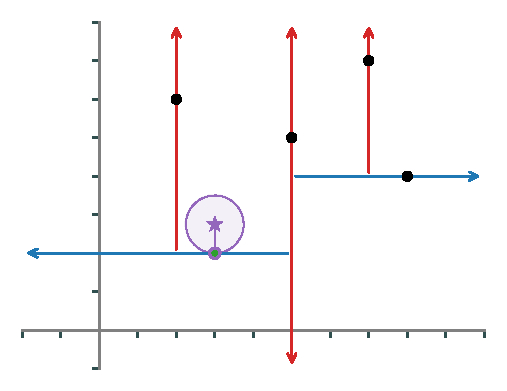
\includegraphics[width=.4\textwidth]{figures/kdtnn_search2.pdf}
    \end{tabular}
    \caption{If the target $\z = [3,2.75]$ were in the tree, it would be to the left of the root, so step left and examine $\x = [3,\textcolor{blue}{2}]$.
    Since $d(\x,\z) < d(\x^*,\z)$, reassign $\x^* = \x$ and recompute $d^*$.
    Now the sphere of radius $d^*$ centered at $\z$ no longer intersects the root's hyperplane, so the nearest neighbor cannot be in the root's right subtree.}
\end{subfigure}
\begin{subfigure}{\textwidth}
    \begin{tabular}{lcr}
    \begin{tikzpicture}[
        baseline=(current bounding box.south),
        level 1/.style={sibling distance=4cm, level distance=1cm},
        level 2/.style={sibling distance=2.5cm, level distance=1cm},
        level 3/.style={sibling distance=1.5cm, level distance=1.5cm},
        edge from parent/.style={draw, ->,thick, >=stealth'}]
        \node [thick,circle,draw] (a) {$[\textcolor{red}{5},5]$}
          child {node[thick,circle,draw=purple] (b) {$[3,\textcolor{blue}{2}]$}
            child {node[draw=none] (invisble) {} edge from parent[draw=none]}
            child {node[draw,thick,circle,fill=green!20!] (c) {$[\textcolor{red}{2},6]$} edge from parent[draw=blue]
              child {node[draw=none] (i) {} edge from parent[draw=none]}}}
          child {node[thick,circle,draw] (g) {$[8,\textcolor{blue}{4}]$}
            child {node[draw=none] (invisible1) {} edge from parent[draw=none]}
            child {node[draw,circle] (e) {$[\textcolor{red}{7},7]$}}};
    \end{tikzpicture}
    &\textcolor{white}{----------}&
    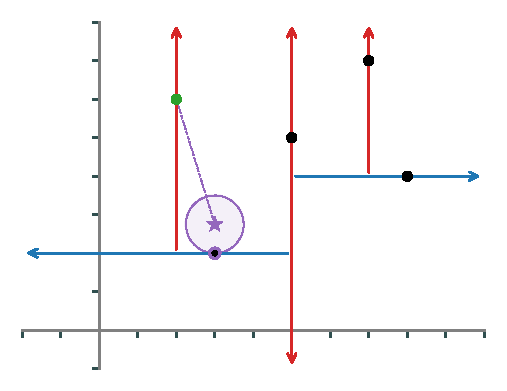
\includegraphics[width=.4\textwidth]{figures/kdtnn_search3.pdf}
    \end{tabular}
    \caption{Continuing the search, step right to check the point $\x = [\textcolor{red}{2},6]$.
    In this case $d(\x,\z) > d(\x^*,\z)$, meaning $\x$ is \textbf{not} nearer to $\z$ than $\x^*$.
    Since $[\textcolor{red}{2},6]$ is a leaf node, retrace the search steps up the tree to check the non-searched branches.
    However, the sphere around $\z$ does not intersect any splitting hyperplanes defined by the tree, so $\x^*$ is guaranteed to be the nearest neighbor.}
\end{subfigure}
\end{center}
\caption{Nearest neighbor search of a $k$-d tree with $k= 2$.
The target is $\z = [3,2.75]$ and the nearest neighbor is $\x^* = [3,\textcolor{blue}{2}]$ with minimal distance $d^* = 0.75$.
The tree structure allows the algorithm to eliminate $[8,\textcolor{blue}{4}]$ and $[\textcolor{red}{7},7]$ from consideration without computing their distance from $\z$.}
\label{fig:nearest-neighbor-query}
\end{figure}

\begin{algorithm}[h] % K-d search algorithm.
\begin{algorithmic}[1]
% \State Let $\z \in \mathbb{R}^k$ be a search target, $d(\cdot,\cdot)$ be a metric, and \texttt{root} be the top of a $k$-d tree. %; \texttt{current} and \texttt{nearest} are \li{KDTNode}s.
\Procedure{Nearest Neighbor Search}{$\z$, \texttt{root}}
\Procedure{KDSearch}{\texttt{current}, \texttt{nearest}, $d^*$}
\If {\texttt{current} \textcolor{blue}{\texttt{is None}}}
    \Comment{Base case: dead end.}
    \State \pseudoli{return} \texttt{nearest}, $d^*$
\EndIf
\State $\x \gets$ \texttt{current.value}
\State $i \gets$ \texttt{current.pivot}
\If {$d(\x,\z) < d^*$}
    \Comment{Check if \texttt{current} is closer to $\z$ than \li{nearest}.}
    \State \texttt{nearest} $\gets$ \texttt{current}
    \State $d^* \gets d(\x,\z)$
\EndIf
\If {$z_i < x_i$}
    \Comment{Search to the left.}
    \State \texttt{nearest}, $d^* \gets$ \texttt{KDSearch}(\texttt{current.left}, \texttt{nearest}, $d^*$)
    \If {$z_i + d^* \ge x_i$}
    \Comment{Search to the right if needed.}
        \State \texttt{nearest}, $d^* \gets$ \texttt{KDSearch}(\texttt{current.right}, \texttt{nearest}, $d^*$)
    \EndIf
\Else
    \Comment{Search to the right.}
    \State \texttt{nearest}, $d^* \gets$ \texttt{KDSearch}(\texttt{current.right}, \texttt{nearest}, $d^*$)

    \If {$z_i - d^* \le x_i$}
    \Comment{Search to the left if needed.}
        \State \texttt{nearest}, $d^* \gets$ \texttt{KDSearch}(\texttt{current.left}, \texttt{nearest}, $d^*$)
    \EndIf
\EndIf
\State \pseudoli{return} \texttt{nearest}, $d^*$
\EndProcedure
\State \texttt{node}, $d^* \gets \texttt{KDSearch}(\texttt{root}, \texttt{root}, d(\texttt{root.value},\z))$
\State \pseudoli{return} \texttt{node.value}, $d^*$
\EndProcedure
\end{algorithmic}
\caption{$k$-d tree nearest neighbor search}
\label{alg:nearest-neighbor-search}
\end{algorithm}

\begin{problem} % K-d nearest neighbor search algorithm.
\label{prob:kdtree-nearest-neighbor-search}
Write a method for the \li{KDT} class that accepts a target point $\z\in\mathbb{R}^k$.
Use Algorithm \ref{alg:nearest-neighbor-search} to solve \eqref{eq:nearest-neighbor-def}.
Return the nearest neighbor $\x^*$ (the actual NumPy array, not the \li{KDTNode}) and its distance $d^*$ from $\z$.

Compare your method to the exhaustive search in Problem \ref{prob:nearest-neighbor-exhaustive-search} and to SciPy's built-in \li{KDTree} class.
This structure is essentially a heavily optimized version of the \li{KDT} class.
To solve the nearest neighbor problem, initialize the tree with data, then ``query'' the tree with the target point.
The \li{query()} method returns a tuple of the minimum distance and the index of the nearest neighbor in the data.

\begin{lstlisting}
>>> from scipy.spatial import KDTree

# Initialize the tree with data (in this example, use random data).
>>> data = np.random.random((100,5))    # 100 5-dimensional points.
>>> target = np.random.random(5)
>>> tree = KDTree(data)

# Query the tree for the nearest neighbor and its distance from 'target'.
>>> min_distance, index = tree.query(target)
>>> print(min_distance)
0.24929868807
>>> tree.data[index]                    # Get the actual nearest neighbor.
array([ 0.26927057,  0.03160271,  0.46830759,  0.26766863,  0.63073275])
\end{lstlisting}
\end{problem}

\begin{warn}
There are a few caveats to using a $k$-d tree for the nearest neighbor search problem.
\begin{itemize}
\item Constructing the tree takes time.
For small enough data sets, an exhaustive search may be faster than the combined time of constructing and searching a tree.
On the other hand, once the tree is constructed, it can be used for multiple nearest-neighbor queries.
\item In the worst case---when the tree is completely unbalanced---the search complexity is $O(km)$ instead of $O(k\log(m))$.
Fortunately, there are algorithms for constructing the tree intelligently so that it is mostly balanced, and a random insertion order usually results in a somewhat balanced tree.
\end{itemize}
% In general, $k$-d trees may be unnecessary or even a hinderance if $X$ is small, but it certainly pays to have a well-constructed $k$-d tree if $X$ is large.
\end{warn}

\section*{K-Nearest Neighbors} % ==============================================

The nearest neighbor algorithm provides one way to solve a common machine learning problem.
In \emph{supervised learning},
% \footnote{In \emph{unsupervised learning} there are no labels provided in the first place.}
a \emph{training set} $X\subset D$ has a corresponding set of \emph{labels} $Y$ that specifies a category for each element of $X$.
For instance, $X$ could contain financial data on $m$ individuals, and $Y$ could be a set of $m$ booleans indicating which individuals have filed for bankruptcy.
Supervised learning algorithms use the training data to construct a function $f:D\rightarrow Y$ that maps points to their corresponding label.
In other words, the algorithm ``learns'' enough about the relationship between $X$ and $Y$ to intelligently label arbitrary elements of $D$.
In the bankruptcy example, a person could then use their own financial data to learn whether or not they look more like someone who files for bankruptcy or someone who does not.

A \emph{$k$-nearest neighbors} classifier uses a simple strategy to label an arbitrary $\z\in D$: find the $k$ elements of $X$ that are nearest to $\z$ (usually in terms of the Euclidean metric) and choose the most common label from those $k$ elements as the label of $\z$.
That is, the points in the $k$ labeled points that are most like $\z$ are allowed to ``vote'' on how $\z$ should be labeled.
See Figure \ref{fig:k-nearest-neighbors}.

\begin{figure}[H]
\begin{tabular}{ccccc}
\begin{tikzpicture}[circ/.style={circle,align=center,minimum size=.5cm}]
    \node[circ,draw=black,thick] (R) {};
    \node[cyan!70,fill=cyan!70,circ,above left=.3cm and .3cm of R] (B1) {};
    \node[cyan!70,fill=cyan!70,circ,below left=-.3cm and .6cm of R] (B3) {};
    \node[yellow!70,fill=yellow!70,circ,below left=.5cm and .6cm of R] (Y1){};
    \node[yellow!60,fill=yellow!60,circ,above right=.3cm and .3cm of R](Y2){};
    \node[yellow!60,fill=yellow!60,circ,below right=0cm and 1cm of R] (Y3) {};
\end{tikzpicture}
%
\quad\qquad\qquad&\qquad\qquad&
%
\begin{tikzpicture}[circ/.style={circle,align=center,minimum size=.5cm}]
    \node[circ,cyan!70,fill=cyan!70,draw=black,thick] (R) {};
    \node[cyan!70,fill=cyan!70,circ,above left=.3cm and .3cm of R] (B1) {};
    \node[cyan!70,fill=cyan!70,circ,below left=-.3cm and .6cm of R] (B3) {};
    \node[yellow!70,fill=yellow!70,circ,below left=.5cm and .6cm of R] (Y1) {};
    \node[yellow!60,fill=yellow!60,circ,above right=.3cm and .3cm of R] (Y2){};
    \node[yellow!60,fill=yellow!60,circ,below right=0cm and 1cm of R] (Y3) {};
    \foreach \a/\b in {R/B1,R/B3,R/Y2} \draw[line width=.05cm] (\a) -- (\b);
\end{tikzpicture}
%
&\qquad\qquad&\qquad\qquad\quad
%
\begin{tikzpicture}[circ/.style={circle,align=center,minimum size=.5cm}]
    \node[circ,yellow!60,fill=yellow!60,draw=black,thick] (R) {};
    \node[cyan!70,fill=cyan!70,circ,above left=.3cm and .3cm of R] (B1) {};
    \node[cyan!70,fill=cyan!70,circ,below left=-.3cm and .6cm of R] (B3) {};
    \node[yellow!70,fill=yellow!70,circ,below left=.5cm and .6cm of R] (Y1) {};
    \node[yellow!60,fill=yellow!60,circ,above right=.3cm and .3cm of R] (Y2){};
    \node[yellow!60,fill=yellow!60,circ,below right=0cm and 1cm of R] (Y3) {};
    \foreach \a/\b in {R/B1,R/B3,R/Y2,R/Y3,R/Y1} \draw[line width=.05cm] (\a) -- (\b);
\end{tikzpicture}
\end{tabular}
\caption{To classify the center node, determine its $k$-nearest neighbors and pick the most common label of the neighbors.
If $k=3$, the $k$ nearest points are two blues and a yellow, so the center node is labeled blue.
For $k=5$, the $k$ nearest points consists of two blues and three yellows, so the center node is labeled yellow.}
\label{fig:k-nearest-neighbors}
\end{figure}

\begin{warn}
The $k$ in $k$-d tree refers to the \textbf{dimension} of the data housed in the tree, but the $k$ in $k$-nearest neighbors refers to the \textbf{number of neighbors} to use in the voting scheme.
Unfortunately, both names are standard.
% The $k$ in the \emph{$k$-means algorithm} refers to the number of clusters to separate the data into.
\end{warn}

\begin{problem} % Write a KNeighborsClassifier class.
\label{prob:kneighbors-classifier}
Write a \li{KNeighborsClassifier} class with the following methods.
\begin{enumerate}
\item The constructor should accept an integer \li{n_neighbors}, the number of neighbors to include in the vote (the $k$ in $k$-nearest neighbors).
Save this value as an attribute.

\item \li{fit()}: accept an $m\times k$ NumPy array $X$ (the training set) and a 1-dimensional NumPy array $\y$ with $m$ entries (the training labels).
As in Problems \ref{prob:nearest-neighbor-exhaustive-search} and \ref{prob:kdtree-nearest-neighbor-search}, each of the $m$ rows of $X$ represents a point in $\mathbb{R}^k$.
Here $y_i$ is the label corresponding to row $i$ of $X$.

Load a SciPy \li{KDTree} with the data in $X$.
Save the tree and the labels as attributes.

\item \li{predict()}: accept a 1-dimensional NumPy array $\z$ with $k$ entries.
Query the \li{KDTree} for the \li{n_neighbors} elements of $X$ that are nearest to $\z$ and return the most common label of those neighbors.
If there is a tie for the most common label (such as if $k=2$ in Figure \ref{fig:k-nearest-neighbors}), choose the alphanumerically smallest label.
\\(Hint: use \li{scipy.stats.mode()}. The default behavior splits ties correctly.)

To get several nearest neighbors from the tree, specify \li{k} in \li{KDTree.query()}.
\begin{lstlisting}
>>> data = np.random.random((100,5))    # 100 5-dimensional points.
>>> target = np.random.random(5)
>>> tree = KDTree(data)

# Query the tree for the 3 nearest neighbors.
>>> distances, indices = tree.query(target, k=3)
>>> print(indices)
[26 30 32]
\end{lstlisting}
\end{enumerate}
\end{problem}

\begin{info}
The format of the \li{KNeighborsClassifier} in Problem \ref{prob:kneighbors-classifier} conforms to the style of \emph{scikit-learn} (\li{sklearn}), a large machine learning library in Python.
In fact, scikit-learn has a class called \li{sklearn.neighbors.KNeighborsClassifier} that is a more robust version of the class from Problem \ref{prob:kneighbors-classifier}.
See \url{http://scikit-learn.org/stable/modules/neighbors.html} for more tools from scikit-learn for solving the nearest neighbor problem in the context of machine learning.
\end{info}

\begin{comment}
To determine the accuracy of a machine learning model, first divide the set of labeled data into a \emph{training set} and a \emph{test set}.
The training set is used to find potentially predictive relationships between the \emph{features}, or individual properties, of a data point.
In the bankruptcy example above, the incomes and debt levels were features of the data.
Relationships between features are discovered in the \emph{training phase} of machine learning.
In the nearest neighbor algorithm, the training phase consists of simply storing the training set.
The test set is a small subset (usually around 20\%) of the original data set.
During the \emph{test phase}, the accuracy of the model is calculated using the test set.
The test set is treated as a set of novel data, and is run through the model.
The model's classifications of the test data are compared to the actual labels of the test data.
The ratio of correct classifications to total number of instances in the test set is the accuracy of the model.

\subsection*{Breaking Ties}
Consider the illustration in Figure \ref{fig:k-nearest-neighbors}.
Suppose that the three neighbors of a new data point were found, but all of these neighbors had different classifications: one neighbor was of class A, one was B, and one was C.
How would the new instance be classified?
A common approach to dealing with ties is to remove the farthest neighbor's vote until a majority vote is found.
In some cases, this results in only the closest neighbor determining the output of a new instance.
\end{comment}

\subsection*{Handwriting Recognition} % ---------------------------------------

\emph{Computer vision} is a challenging area of artificial intelligence that focuses on autonomously interpreting images.
Perhaps the simplest computer vision problem is that of translating images into text.
Roughly speaking, computers store grayscale images as $M \times N$ arrays of pixel brightness values: 0 corresponds to black, and 255 to white.
Flattening out such an array yields a vector in $\mathbb{R}^{MN}$.
Given some images of characters with labels (assigned by humans), a $k$-nearest neighbor classifier can intelligently decide what character the image represents.

\begin{problem}
The file \texttt{mnist\_subset.npz} contains part of the MNIST dataset,\footnote{See \url{http://yann.lecun.com/exdb/mnist/}.} a collection of $28\times 28$ images of handwritten digits and their labels.
The data is split into four parts.
\begin{itemize}
\item \li{X_train}: A $3000\times 728$ matrix, the training set.
Each of the $3000$ rows is a flattened $28\times 28$ image to be used in training the classifier.

\item \li{y_train}: A 1-dimensional NumPy array with $3000$ entries.
The entries are integers from 0 to 9, the labels corresponding to the images in \li{X_train}.

\item \li{X_test}: A $500\times 728$ matrix of $500$ images to classify.

\item \li{y_test}: A 1-dimensional NumPy array with $500$ entries.
These are the labels corresponding to \li{X_test}, the ``right answers'' that the classifier will try to guess.
\end{itemize}
The following code uses \li{np.load()} to extract the data.
% Use \li{np.load()} to extract the data.
% An \texttt{npz} file holds several arrays, which can be accessed like the values of a dictionary.
\begin{lstlisting}
>>> data = np.load("mnist_subset.npz")
>>> X_train = data["X_train"].astype(np.<<float>>)          # Training data
>>> y_train = data["y_train"]                           # Training labels
>>> X_test = data["X_test"].astype(np.<<float>>)            # Test data
>>> y_test = data["y_test"]                             # Test labels
\end{lstlisting}
To visualize one of the images, reshape it as a $28\times 28$ array and use \li{plt.imshow()}.
\begin{lstlisting}
>>> from matplotlib import pyplot as plt
>>> plt.imshow(X_test[0].reshape((28,28)), cmap="gray")
>>> plt.show()
\end{lstlisting}
\begin{center}
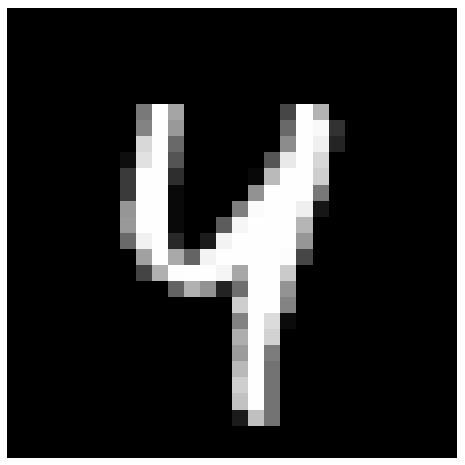
\includegraphics[width=.15\textwidth]{figures/digit.pdf}
\end{center}

% \begin{figure}[H]
% \centering
% 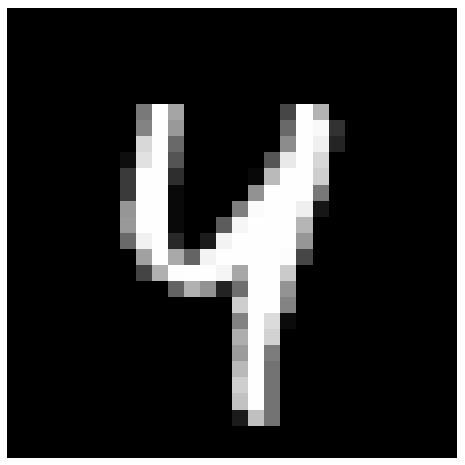
\includegraphics[width=.4\textwidth]{figures/digit.pdf}
% \caption{The number 6 taken from the data set.}
% \label{fig:digit}
% \end{figure}

Write a function than accepts an integer \li{n_neighbors}.
Load a classifier from Problem \ref{prob:kneighbors-classifier} %or a \li{sklearn.neighbors.KNeighborsClassifier}
with the data \li{X_train} and the corresponding labels \li{y_train}.
Use the classifier to predict the labels of each image in \li{X_test}.
Return the classification accuracy, the percentage of predictions that match \li{y_test}.
The accuracy should be at least $90\%$ using $4$ nearest neighbors.
\end{problem}

\begin{info}
The $k$-nearest neighbors algorithm is \textbf{not} the best machine learning algorithm for this problem, but it is a good starting point because of its simplicity.
In fact, $k$-nearest neighbors is often used as a baseline to compare against more complicated machine learning techniques.
\end{info}

\newpage

\section*{Additional Material} % ==============================================

\subsection*{Ball Trees} % ----------------------------------------------------

The nearest neighbor problem can also be solved efficiently with a \emph{ball tree}, another space-partitioning data structure.
Instead of separating $\mathbb{R}^k$ by hyperplanes, a ball tree uses nested hyperspheres to split up the space.
Since the partitioning scheme is different, a nearest neighbor search through a ball tree is more efficient than the $k$-d tree search for some data sets.
See \url{https://en.wikipedia.org/wiki/Ball_tree} for more details.

\subsection*{The Curse of Dimensionality} % -----------------------------------

The \emph{curse of dimensionality} refers to a phenomena that occurs when dealing with high-dimensional data: the computational cost of an algorithm increases much more rapidly as the dimension increases than it does when the number of points increases.
This problem occurs in many other areas involving multi-dimensional data, but it is quite apparent in a nearest neighbor search.

\begin{figure}[H] % Curse of Dimensionality
\captionsetup[subfigure]{justification=centering}
\centering
\begin{subfigure}{.49\textwidth}
    \centering
    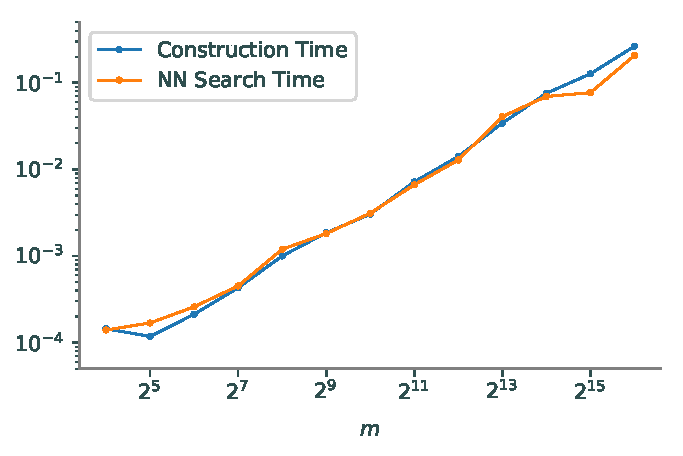
\includegraphics[width=\textwidth]{figures/curse_m.pdf}
    \caption{Fixing $k$ and increasing $m$ leads to consistent growth in execution time.}
\end{subfigure}
%
\begin{subfigure}{.49\textwidth}
    \centering
    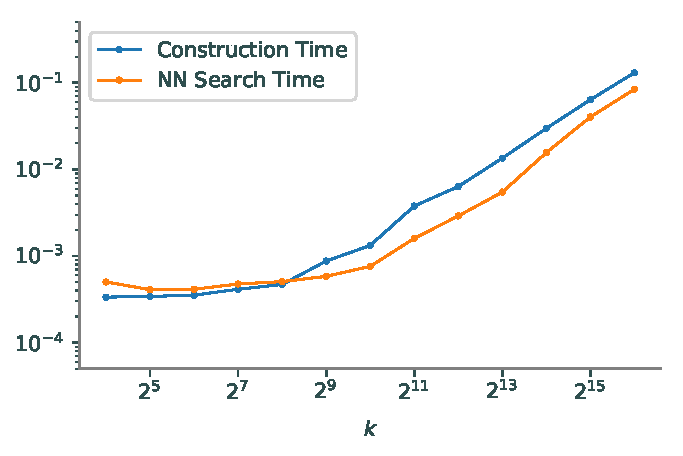
\includegraphics[width=\textwidth]{figures/curse_k.pdf}
    \caption{For fixed $m$, the times takes a sharp upturn around $k = 2^9$ relative to previous growth rates.}
\end{subfigure}
\caption{Construction and nearest neighbor search times for a $k$-d tree with a $m\times k$ training set.}
\end{figure}

See \url{https://en.wikipedia.org/wiki/Curse_of_dimensionality} for more examples.
One way to avoid the curse of dimensionality is via \emph{dimension reduction}, a process usually based on the singular value decomposition (SVD) that projects data into a lower-dimensional space.

\subsection*{Tiebreaker Strategies} % -----------------------------------------

As mentioned in Problem \ref{prob:kneighbors-classifier}, the majority voting scheme in the $k$-nearest neighbor algorithm can often result in a tie.
Breaking the tie intelligently is a science unto itself, but here are a few common strategies.
\begin{enumerate}
\item For binary classification (meaning there are only two labels), choose an odd $k$ to avoid a tie in the first place.
\item Redo the search with $k-1$ neighbors, repeating as needed until $k=1$.
\item Choose the label that appears more frequently in the test set.
\item Choose randomly among the labels that are tied for most common.
\end{enumerate}

\subsection*{Additional Code} % -----------------------------------------------

The following code creates a string representation for the \li{KDT} class.
Use this to test Problem \ref{prob:kdt-insert}.

\begin{lstlisting}
class KDT:
    # ...
    def __str__(self):
        """String representation: a hierarchical list of nodes and their axes.

        Example:                           'KDT(k=2)
                    [5,5]                   [5 5]   pivot = 0
                    /   \                   [3 2]   pivot = 1
                [3,2]   [8,4]               [8 4]   pivot = 1
                    \       \               [2 6]   pivot = 0
                    [2,6]   [7,5]           [7 5]   pivot = 0'
        """
        if self.root is None:
            return "Empty KDT"
        nodes, strs = [self.root], []
        while nodes:
            current = nodes.pop(0)
            strs.append("{}\tpivot = {}".<<format>>(current.value, current.pivot))
            for child in [current.left, current.right]:
                if child:
                    nodes.append(child)
        return "KDT(k={})\n".<<format>>(self.k) + "\n".join(strs)
\end{lstlisting}
